Before deeper concepts, algorithms and application of undirected graphical models are illustrated, some basics of those models need to be explained. For instance the formal definition of undirected graphs as well as their parameterization.

\subsection{Definition}

As other graphical models like the Bayesian network the undirected graphical network consists of a set of nodes $V$ (also called vertices) and a set of edges between the nodes $E$, which is a set of tuples of exactly two nodes. The key difference to a Bayesian network is that those edges are not directed, in the meaning that the dependency between two nodes do not have a direction, as described in \cite{koller2009probabilistic}.

When the edges of a undirected graph represent random variables, it is called a undirected graphical model or also Markov network or Markov random field.\cite{kindermann1980markov} The edges hereby represent a probabilistic dependency between the linked random variables.

To be considered as a Markov network (or Markov random field) the random variables need to satisfy the following Markov properties with respect to the graph, as described in \cite{markov1957theory}:

\begin{enumerate}
\item Pairwise Markov property: Given all other random variables two non-adjacent (which means there is no edge between those two nodes) variables are conditionally independent.
\item Local Markov property: Given all its neighbors a random variable is conditionally independent of all other non-adjacent random variables.
\item Global Markov property: Any two subsets are conditionally independent if any path between them passes through a given third subset which is disjoint to those both.  
\end{enumerate}


Figure \ref{fig:basic} shows a simple example of an graphical model (Markov network) with a set of four random variables $V=\{A,B,C,D\}$ and four probabilistic dependencies (edges): $E=\{(A,B),(B,C),(A,C),(C,D)\}$. In this example, the nodes could represent humans and the edges could represent a probabilistic presentation of how like it is, that two persons are relatives. Based on such a model the probability of how likely it is that all four persons are relatives could be calculated. To do so, it is necessary to parameterize the model.

\begin{figure}[htpb]
  \centering
  	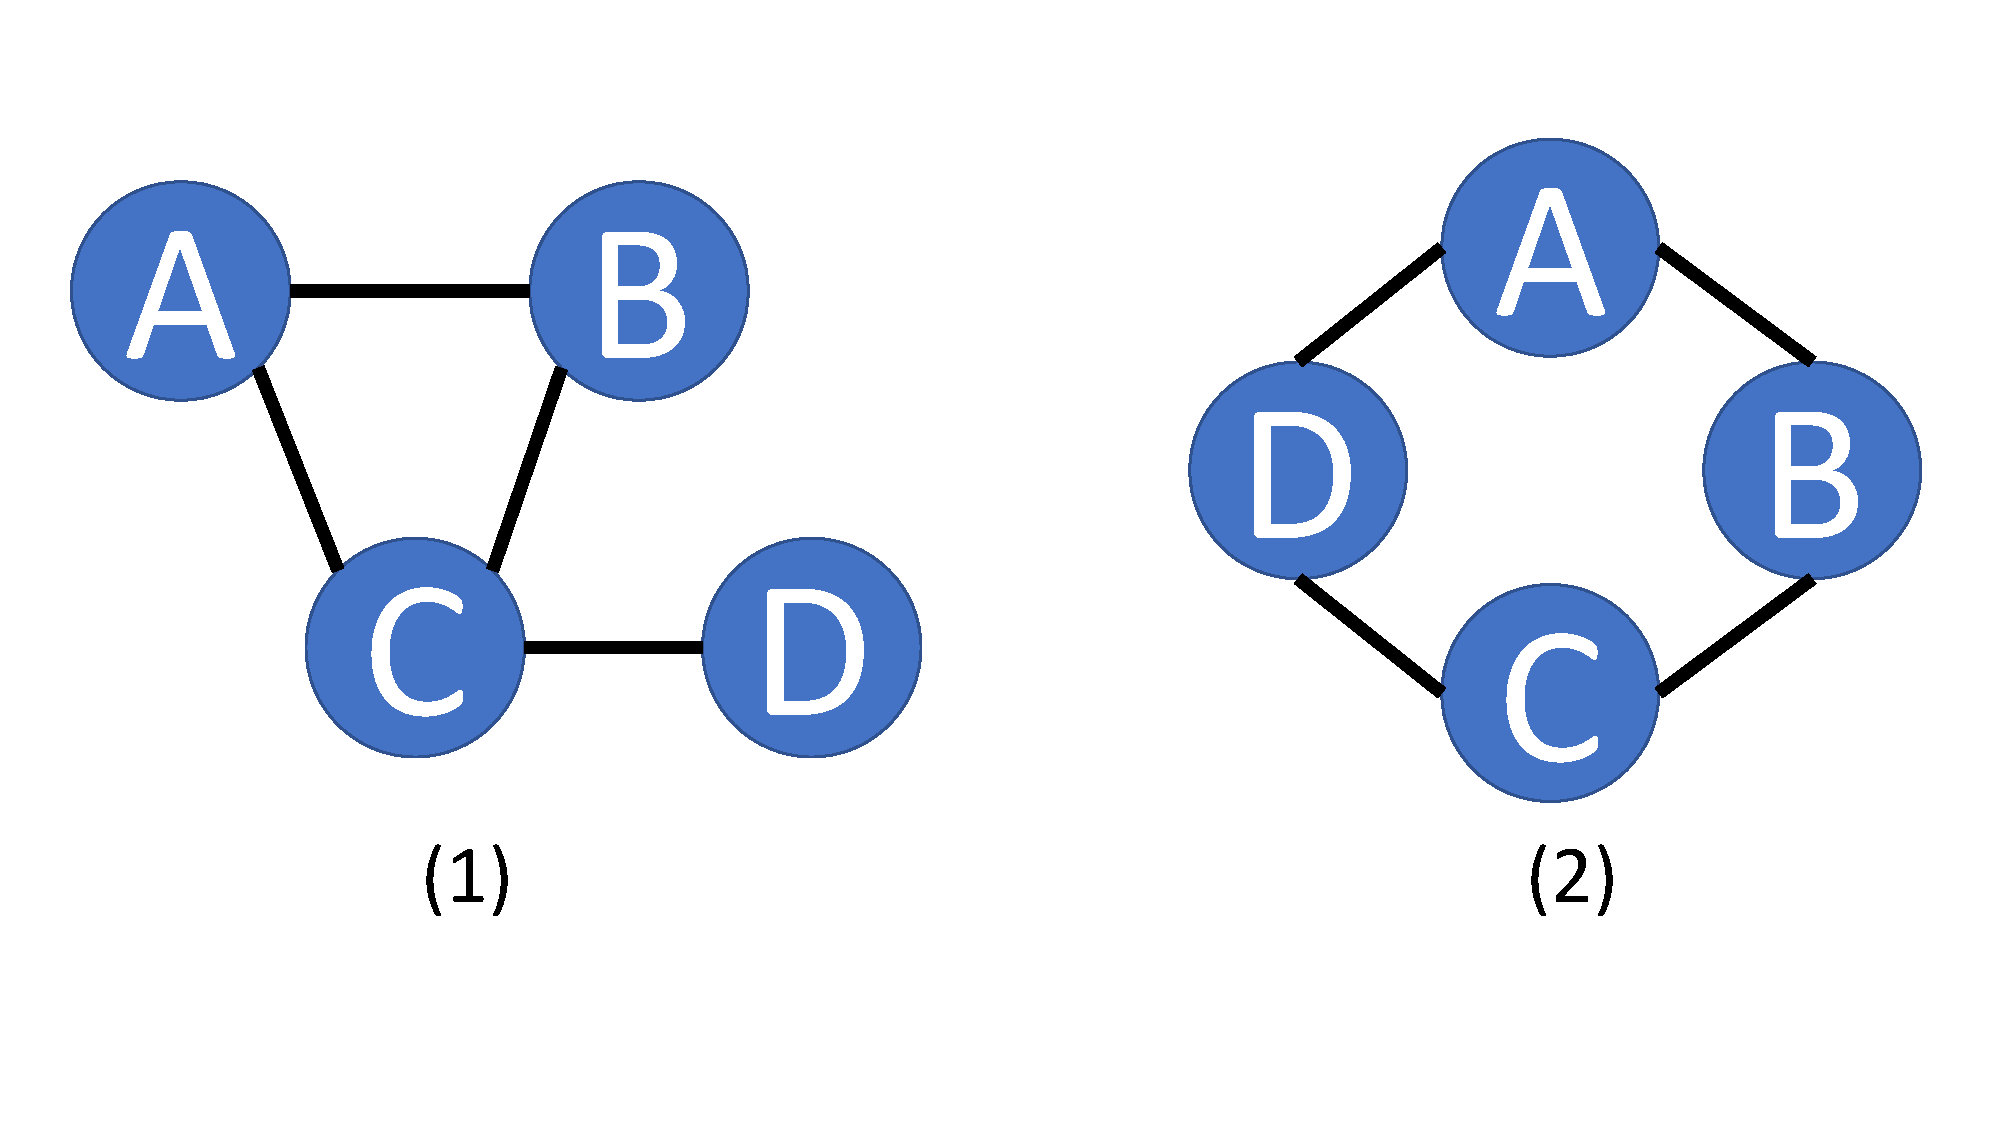
\includegraphics[scale=0.3]{img/basic.pdf} 
  \caption{Simple Undirected Graphical Model}
  \label{fig:basic}
\end{figure}

TODO: when the joint probability is strictly positive than it is a Gibbs random field cause it can be represented by the Gibbs measure


\subsection{Parameterization}

TODO: clique \\
TODO clique factorization

In order to calculate propabilities on an undirected graphical model, the model needs to be parameterized in the first place. Such a parameterization is achieved by assigning factors to subsets of random variables of the graph. Each factor consists of parameters, which assing a real number to a certain combination of values the included random variables can adapt. If for example there is a factor over two binary random variables $A$ and $B$ the factor $\phi(A,B)$ would have four parameters for each combination of values of $A$ and $B$. Figure \ref{fig:param} shows such a factor and demonstrate the assignment of probabilities to each possible combination. If the assigned real numbers represent probabilities and not any kind of unnormalized score, they sum up to one, as shown in the figure. 

In order to parameterize the edges between the nodes (means the relation between the random variables) functions, called factors, are defined. 


TODO: factors - unnormalized/normalized


TODO: How does the method work? What are the appealing properties?
